\documentclass[12pt]{article}

\usepackage[utf8]{inputenc}
\usepackage[a4paper, margin=1in]{geometry}
\usepackage{booktabs}
\usepackage{physics}
\usepackage{amsmath}
\usepackage{amsfonts}
\usepackage{graphicx}
\usepackage{siunitx}
\usepackage{multirow}

\graphicspath{{./figures}}

\title{Physical Climatology (AES 630) Final}
\author{Mitchell Dodson}
\date{December 6, 2023}

\newcommand*{\problem}[2]{
    \begin{table}[ht]
    \centering
        \begin{tabular}{ | p{.1\linewidth} p{.9\linewidth} | }
            \hline
            \vspace{.3em}\textbf{\large#1:} & \vspace{.3em}\footnotesize{#2}\hspace{.2em}\vspace{.5em} \\ \hline
        \end{tabular}
    \end{table}
}


\newcommand\T{\rule{0pt}{2.6ex}}       % Top strut
\newcommand\B{\rule[-1.2ex]{0pt}{0pt}} % Bottom strut

\begin{document}

\vspace{-2em}

\maketitle

\vspace{-2em}

\section{EBM Problem}

\begin{figure}[h!]
    \centering
    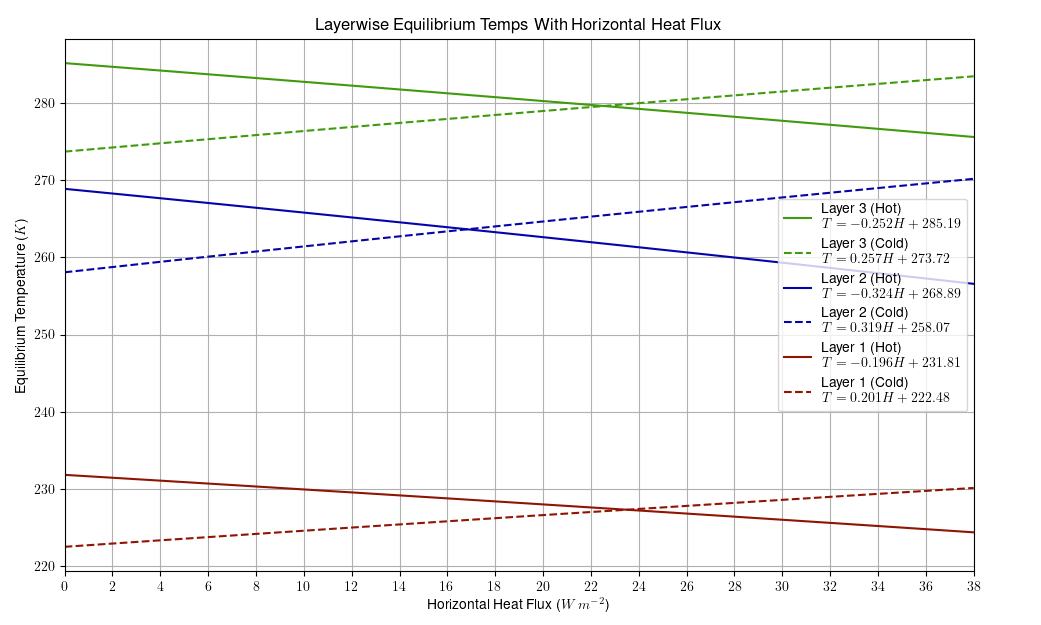
\includegraphics[width=.98\linewidth]{q1.png}

    \vspace{1em}

    \begin{tabular}{c | c c c | c c c}
        & Layer 1 & Layer 2 & Layer 3 & $\frac{dT_1}{dH}$ & $\frac{dT_2}{dH}$ & $\frac{dT_3}{dH}$ \B\\
        \hline
        Hot World & 231.809 & 268.891 & 285.192 & -0.196 & -0.324 & -0.252 \T\\
        Cold World & 222.480 & 258.070 & 273.715 & 0.201 & 0.319 & 0.257 \\
    \end{tabular}

    \caption{Equilibrium temperatures of ``hot world'' with $Q_H = 330\,\si{W.m^{-2}}$ and ``cold world'' with $Q_C = 280\,\si{W.m^{-2}}$ as horizontal heat flux from the hot to the cold world's troposphere increases up to $38\,\si{W.m^{-2}}$. The table shows the initial layerwise temperatures as well as their linear rates of change with respect to the heat flux.}
    \label{q1}
\end{figure}

\begin{equation}\label{conduit}
    \begin{split}
        T_{3C} &= T_{3H} \\
        -0.252\,H + 285.19 &= 0.257\,H + 273.72 \\
        H &= 22.53\,\si{W.m^{-2}}\\
    \end{split}
\end{equation}

Figure \ref{q1} shows the effects on each layer's equilibrium temperature as the exchange of heat between the hot and cold worlds increases, and Equation \ref{conduit} sets each planet's linear approximation of the surface temperature response equal to each other in order to determine their intersection. My results show that the conduit between each world's troposphere must transmit $H=22.53\,\si{W.m^{-2}}$ of heat flux in order to maintain the same surface temperature between the two systems.

\begin{equation}\label{instability}
    \begin{split}
        T_{3H} = T_{3C} &= 0.257 \cdot 22.53 + 273.72 = 279.51\,\si{K} \\
        T_{2H} &= -0.324 \cdot 22.53 + 268.89 = 261.59\,\si{K} \\
        T_{2C} &= 0.319 \cdot 22.53 + 258.07 = 265.26\,\si{K} \\
    \end{split}
\end{equation}

Equation \ref{instability} shows the equilibrium temperatures of layers 2 and 3 for both planets at the surface temperature intersection, given their linear approximations. These suggest that in the cold planet the temperature difference between the surface and the troposphere is $T_{3C}-T_{2C} = 14.25\,\si{K}$, and in the hot planet the temperature difference is $T_{3H}-T_{2H} = 17.92\,\si{K}$. Assuming layer 2 is the same altitude from the surface for both planets, this indicates that the addition of heat to the cold planet's troposphere weakens its lapse rate relative to the hot planet. The result is that less potential energy is available for buoyant air parcels to be lofted from the cold planet, which correlates with less overall vertical heat flux for that planet. The inverse is true for the hot planet, which has a relatively steep lapse rate that may enhance the rate at which vertical heat flux redistributes energy from the surface layers to the troposphere. Furthermore, the absolute magnitudes of $\frac{dT_2}{dH}$ are greater than those of $\frac{dT_3}{dH}$ in both planets' cases. This suggests that after implementing the heat conduit, the hydrostatic instability of the hot planet increases and the cold planet becomes more stable compared to their original lapse rates.

\section{Climate Sensitivity and Politics}

\noindent\textbf{Part A}

\begin{equation}\label{sb1}
    T_s = \sqrt[4]{\frac{S_0 (1-\alpha_p)}{4 \sigma}} = \sqrt[4]{\frac{1365 (1-0.31)}{4 \sigma}} = 253.85\,\si{K}
\end{equation}

\begin{equation}\label{sb2}
    \frac{d E}{d T_s} =  \frac{d}{dT_s}(\sigma T_s^4) = 4\sigma T_s^3 = 4 \sigma (253.85\,\si{K})^3 = 3.71\,\si{W.m^{-2}.K^{-1}}
\end{equation}

\begin{equation}\label{sb3}
    \lambda_R = \frac{d T_s}{d E} = \frac{1}{3.71} = 0.2695\,\si{K.(W.m^{-2})^{-1}}
\end{equation}

The Stefan-Boltzmann feedback with no atmosphere describes a planetary energy system with a surface temperature that only depends on the amount of insolation that is attenuated by the surface, which is modulated by the solar constant $S_0 = 1365\,\si{W.m^{-2}}$ and the surface's albedo (and by extension its absorptivity/emissivity). Equation \ref{sb1} shows that the surface temperature in this model is $253.85\,\si{K}$ assuming Earth's approximate albedo of $\alpha_p = 0.31$.

Equation \ref{sb2} characterizes the change in the planet's radiant exitance with respect to surface temperature in terms of the Stefan-Boltzmann law. If we were modeling the actual radiative power of the surface it would be more appropriate to include an emissivity coefficient $\epsilon_p = 1-0.31 = 0.69$, however for the sake of this question I assume the surface radiates as a blackbody as a standard for reference. Inverting this equation to express the change in surface temperature with respect to the radiant exitance, Equation \ref{sb3} shows that the climate sensitivity given only the Stefan-Boltzmann feedback for a planet with no atmosphere is $\lambda_R = 0.2695$.

\vspace{2em}\noindent\textbf{Part B}

\begin{equation}\label{q2b1}
    \sigma T_a^4 = \sigma T_e^4 = \frac{S_0}{4}(1-\alpha_p) = Q
\end{equation}

\begin{equation}\label{q2b2}
    \begin{split}
        \sigma T_s^4 &= \sigma T_a^4 + \frac{S_0}{4}(1-\alpha_p) = 2Q \\
        T_s &= \sqrt[4]{\frac{2Q}{\sigma}}
    \end{split}
\end{equation}

In a planetary system with a single thermally-opaque atmospheric layer, the equilibrium emissive power of the planet equals that of the atmospheric layer, as Equation \ref{q2b1} shows. The energy balance at the surface is expressed by Equation \ref{q2b2}, which indicates that outgoing longwave flux from the surface $\sigma T_s^4$ is balanced by downward longwave emissions from the atmospheric layer as well as shortwave solar irradiance.

\begin{equation}\label{q2b3}
    \begin{split}
        \frac{dT_s}{dQ} &= \frac{d}{dQ}\left(\sqrt[4]{\frac{2Q}{\sigma}}\right) \\
        &= \frac{1}{4} Q^{-\frac{3}{4}} \left(\frac{2}{Q}\right)^{\frac{1}{4}} \\
        &= \frac{1}{4} (\sigma T_e^4)^{-\frac{3}{4}} \left(\frac{2}{\sigma}\right)^{\frac{1}{4}} \\
        &= \frac{\sqrt[4]{2}}{4\sigma}T_e^{-3} \\
        &= \lambda_R = \frac{\sqrt[4]{2}}{4\sigma}253.85^{-3} \approx 0.321\,\si{K.{W.m^{-2}}^{-1}} \\
    \end{split}
\end{equation}

Equation \ref{q2b3} shows that the combined solar and atmospheric radiation incident on the surface results in a higher climate sensitivity in response to an increment change in solar irradiance absorbed by the planet.

\vspace{2em}\noindent\textbf{Part C}

\begin{equation}\label{q2b4}
    \begin{split}
        Q &= \frac{S_0}{4}(1-\alpha_p) = \sigma T_e^4 = A+BT_s \\
        \frac{dQ}{dT_s} &= B \\
        \lambda &= \frac{dT_s}{dQ} = \frac{1}{B} \\
    \end{split}
\end{equation}

Equation \ref{q2b4} shows the water vapor feedback given that the outgoing energy response is linear with respect to surface temperature. In contrast to other climate sensitivity models which have a fractional exponential relationship with temperature, the water vapor feedback is a decent approximation that reflects the strong greenhouse effect of atmospheric water vapor, and the exponential dependence of saturation mixing ratio on air temperature. Assuming relative humidity remains consistent as air temperature rises, the total material capacity of water vapor that can be sustained before condensing increases rapidly.

\vspace{2em}\noindent\textbf{Part D}

Carbon dioxide has a mixing ratio that is nearly homogeneous throughout the atmosphere vertically, zonally, and meridionally. The direct effect of an increase in CO$_2$ is enhanced attenuation and subsequent re-emission of solar irradiance near the $2\,\si{\mu m}$ and $2.7\,\si{\mu m}$ spectral bands, and of planetary emissions around $4.3\,\si{\mu m}$ and $15\,\si{\mu m}$. The direct shortwave effects of CO$_2$ are relatively insignificant for the climate system since the gas' shortwave absorption lines aren't near the peak of the solar emission curve. In the longwave infrared range, however, CO$_2$ plays a considerable role as a greenhouse gas because its $15\,\si{\mu m}$ absorption bands are very near the peak of the Earth's thermal emission curve. This range of absorption by CO$_2$ is nearly saturated, which means that effectively all of Earth's emissions in this range are attenuated. Thus, the effect of an increase in concentration is to decrease the distance that the average photon emitted by the surface can travel before being absorbed. In other words, raising CO$_2$ levels throughout the atmosphere especially promotes warming near the surface by decreasing the path length of infrared emissions. This effect may be compounded by the fact that this spectral range shares absorption lines with other atmospheric constituents, mainly H$_2$O and O$_2$.

In addition to the radiative feedbacks from CO$_2$ which can increase surface warming, another major positive feedback is the increased presence of water vapor in the troposphere as temperatures increase. This is because per the Clausius-Clapeyron equation, the saturation mixing ratio of water vapor increases rapidly with temperature. As a result, moist air can hold considerably more water vapor before becoming saturated and condensing. Since water vapor is a very strong greenhouse gas, the effect is to increase the amount of back-radiation from the atmosphere incident on the surface, effectively retaining heat in the troposphere and increasing its equilibrium temperature.

Finally, tropospheric warming from the above feedback mechanisms causes the boundary of the polar ice caps to shift poleward. Since ice has an extremely high albedo, reduction in the surface area of ice decreases the planetary albedo, which in turn increases the amount of insolation retained by Earth's energy system.

\vspace{2em}\noindent\textbf{Part E}

The positive feedbacks from increasing the atmospheric mixing ratio of CO$_2$ in Part D are offset by several negative feedbacks that mitigate the sensitivity of Earth's climate system. The most straightforward of these is the Stefan-Boltzmann effect, which states that an increase in an object's temperature also increases the emissive power of that object. This means that a warming atmosphere also emits more longwave radiation back into space, so the atmosphere's equilibrium temperature is cooler than it would be if the Earth continued to lose energy at the original rate.

Perhaps the most considerable and uncertain negative feedback at play in the climate system is the type and distribution of clouds in the troposphere. Due to their high shortwave reflectivity and thermal emissivity, the presence of clouds in an atmospheric column generally cause cooling by increasing the amount of radiation leaving Earth. Relevant cloud features that effect their forcing amounts include their altitude, optical depth, and the effective radii of their constituent particles. Cold and optically-thin cirrus clouds don't reflect very much shortwave radiation, but have a longwave greenhouse effect. Water clouds like stratus and stratocumulus have similar emission temperatures to surface water, and are incredibly reflective, especially if their composition favors smaller cloud particles. Although the responses of the distributions of these clouds properties to changing tropospheric temperatures (and other secondary effects) isn't well understood, a roughly 10$\%$ increase in the total cloud cover would be enough to offset all of the above positive climate feedbacks.

Finally, the above cloud effects may be exacerbated by other factors, notably the presence of cloud condensation nuclei like dust and oceanic particulate emissions. In the latter case, an increase in ocean temperatures resulting from the CO$_2$ forcing may have the secondary effect of increasing the rate at which biological elements emit sulfate aerosols, which diffuse into the troposphere and act as efficient cloud condensation nuclei. This decreases the average effective radius of cloud particles, which makes clouds even more reflective and increases the clouds' lifetime.

\vspace{2em}\noindent\textbf{Part F}

Although I haven't personally read much of the background literature informing modern climate models, my understanding is that they necessarily make a series of assumptions and parameterizations that cause them to meaningfully disagree with each other. Since these forcings are so dynamically entangled with each other, in my opinion it seems likely that even small amounts of model error could have major effects on predictions, and may even call into question the accuracy of error characterization within the model.

I believe, in general, that an individual's as well as humanity's ability to interpret and characterize Reality in almost any domain is hopelessly inadequate, and that we perpetually overestimate the fidelity of our understanding, especially when we have skin in the game. Although I believe we over-value our beliefs, I also believe we often \textit{under-value} our perception, as well as mistake our beliefs for perception. Furthermore, I think information untainted by belief is the most valuable thing in the universe to a being that wants to understand Reality.

This is to say that the field of climatology is cursed by the impossibility of its task, and more recently by that objectivity is tainted by people's beliefs having stake in the matter. It saddens me to see scientists on either ``side'' of the climate question because I don't have the time or intelligence to fully vet all of their claims. I'm forced to assume that anything I learn which isn't almost directly observational has passed through a distorting filter of idealogical disposition in addition to the de-facto distorting filter of scientific characterization, and that I naturally inherit their biases despite my best efforts.

Nonetheless, I have much hope because climatology is a field which is uniquely blessed to be absolutely \textit{drowning} in observational information. We have vastly more data than we have the capacity to use, and with time our ability to use our instruments to perceive Reality and assimilate information only increases in scope, volume, resolution, and confidence. Although we may not be able to model climate feedbacks with the confidence and accuracy we desire, I think there is still much truth to uncover by observing them.

\vspace{2em}\noindent\textbf{Part G}

The only issue I think the articles provide evidence for is that there is discord in the community of climatologists on the magnitude of climate change and the extent to which anthropogenic factors contribute to the change. In terms of scientific questions, I wouldn't even consider the foundations of science -- for example the Copernican principle or the time-invariance of the laws of physics -- to be ``settled''. All I know is that I know nothing.

The problem of communicating uncertainty in science to the public is an insidious one because (1) the public will likely ignore significant information if it is presented with a lack of confidence, especially in an age when only sensational claims are propagated and heard (2) uncertainty is inevitable, and the level of confidence at which a belief is actionable is perpetually subjective and (3) in my experience scientists themselves often have quiet voices unless they sacrifice their integrity, so the truest findings often either fall on deaf ears, or are only heard once they are distorted by others who have louder voices and their own incentives.

Nonetheless, in the ``digital age'' I believe many in the public are starving for truth, and that curious people are becoming increasingly cognizant of the untruth of digital noise. Furthermore, I believe people who learn in good faith can naturally hone their ability to evaluate the truth-quality of information they receive. One profound benefit of the digital age is that people have unprecedented practical access to information, both true and untrue. As such, it is incumbent upon scientists to honestly cultivate the trust of the public by producing free information that is comprehensible, useful, and accurate at all levels of background knowledge. I think one of the quickest ways for a scientist to lose the trust of the public is to use their platform and resources to meddle in political affairs. If a scientist uses their knowledge to leverage ambiguous beliefs regarding the public good in a social/geopolitical sense, as a member of the public I personally take it as observational evidence that their truth-claims are colored -- if not compromised --  by the bottomless subjectivity and intractable tangle of ingenuine perspectives that constitute politics.

My impression of the original al.com article is that it aims to characterize Dr. John Christy as a genuine scientist whose work led him to be swept into the tides of politics. The quotations from other scientists generally come across as unsubstantiated and personal, and the author indeed invokes but doesn't support the a-priori assumption that Dr. Christy's perspective is incorrect, and there seem to be an abundance of unfair subtextual suggestions that Dr. Christy (and perhaps UAH as an institution) are bending to religious, political, and financial forces rather than scientific integrity. If the goal of the piece was to provide truthful information in an objective way, it certainly failed. Nonetheless, the writing style and interjections of personal characterizations of Dr. Christy make it clear to me that precise science communication is not the goal; it's a literary character piece. Narratives can never capture the essence of a person, and make a poor medium for science communication. Although it's unfortunate that Dr. Christy was unfairly neglected the ability to respond to criticism within the article, I can understand why it was written by adopting the perspective of journalist who has only ever heard information contrary to Dr. Christy's claims, and just wants to write a compelling story.

Dr. Christy's response has a much higher informational value because it was written with the rhetorical goal of addressing specific ambiguous or inaccurate claims made by the prior article. The response does a good job of providing detailed context which is much easier to follow than the original publication.

\section{Tropical SST}

\begin{figure}[h!]
    \centering
    \makebox[\textwidth]{
        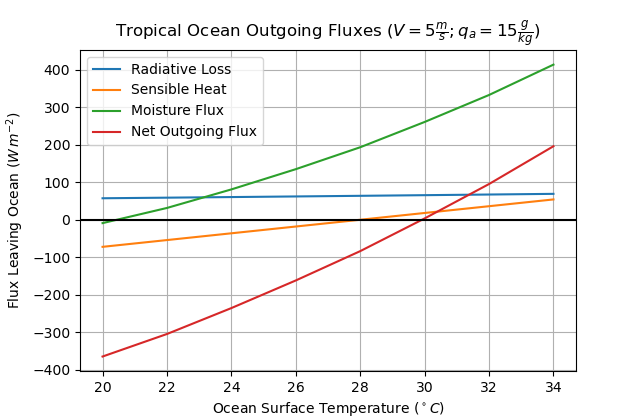
\includegraphics[width=.55\linewidth]{q3a.png}
        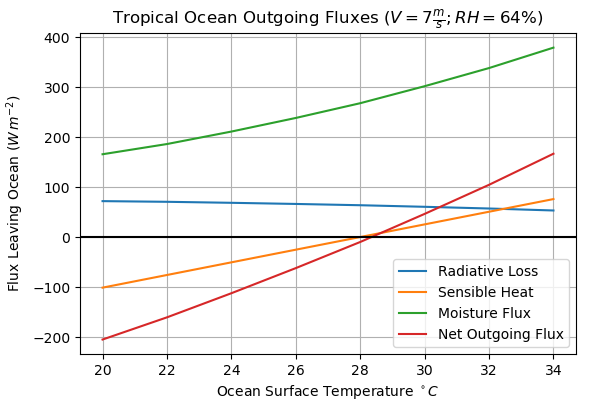
\includegraphics[width=.55\linewidth]{q3b.png}
    }
    \caption{Magnitude of relevant energy fluxes leaving the tropical ocean surface given bulk approximations. Includes approximations with a wind speed $V = 5\,\si{m.s^{-1}}$ and atmospheric water vapor mixing ratio $q_a = 15\,\si{g.kg^{-1}}$ (left) and with wind speed $V = 7 \,\si{m.s^{-1}}$ and relative humidity $RH=64\%$ (right).}\label{seaflux}
\end{figure}

Figure \ref{seaflux} displays the contributions of several fluxes from the tropical ocean, such that positive values correspond to a net energy loss from the ocean. The entire system consists of insolation absorbed by the ocean surface, net longwave back radiation between outgoing and incoming emissions, sensible heat fluxes from eddies (proportional to the difference in ocean and atmospheric temperature), and latent heat fluxes also from eddies (proportional to the difference in mixing ratio).

Although the energy contributed by solar irradiance isn't included in the flux diagrams of Figure \ref{seaflux}, it is by far the most substantial source of energy to the ocean surface which is offset by the other fluxes. The absorbed insolation assuming that there are no reflecting species in the atmospheric column is approximately $F^\downarrow_{abs} = Q_{TOA} \cdot (1-a_{a}) \cdot (1-\alpha_o) = 412\,\si{W.m^{-2}} \cdot (1-0.1) \cdot (1-0.08) = 341.136\,\si{W.m^{-2}}$, where $a_a$ is the shortwave atmospheric absorptivity and $\alpha_o$ is the shortwave ocean albedo.

The latent (moisture) flux starts small (and slightly negative) when the ocean surface is $20\,\si{^\circ C}$ because the sea surface mixing ratio is slightly lower than the atmospheric mixing ratio, but outgoing moisture flux increases rapidly with the surface temperature because of enhanced evaporation rates associated with the warmer water, and the gradual reduction in relative humidity with respect to the constant atmospheric mixing ratio $q_a=15\,\si{g.kg^{-1}}$.

The radiative heat loss is a net loss for the ocean, and slightly increases in magnitude from $57.3\,\si{W.m^{-2}}$ to $69.1\,\si{W.m^{-2}}$ in the observed temperature range. The change is due to the emissive power of the ocean increasing as its temperature does per the Stefan-Boltzmann law. Nonetheless, the magnitude of this change is rather small because increases in outgoing radiant exitance from the ocean are somewhat offset by enhanced thermal re-emission by the atmosphere.

Finally, the sensible heat flux is proportional to the difference between the atmosphere and ocean temperature, so it only becomes positive once the ocean temperature exceeds the atmospheric temperature at $28\,\si{^\circ C}$. This phenomena corresponds to the rebalancing of thermal energy between adjacent surfaces by conduction through mixing, driven by vertical eddies.

In total, the net flux from the ocean becomes positive (outgoing) at a surface temperature of about $30\,\si{^\circ C}$, as indicated by the red line in Figure \ref{seaflux}. At this point, all of the fluxes except for incoming solar energy serve to remove energy from the ocean. Moreover, the magnitude of insolation was calculated with the assumption that there are no reflective species like clouds or aerosols in the atmosphere. Since an increase in atmospheric column albedo would have a net cooling effect, we can comfortably conclude that the sea surface is unlikely to receive enough energy to bring its temperature far past this $30\,\si{^\circ C}$ mark under normal circumstances.

The right-side image in Figure \ref{seaflux} demonstrates the changes in the energy system due to an increase in wind speed from $5\,\si{m.s^{-1}}$ to $7\,\si{m.s^{-1}}$, and a fixed relative humidity of $RH=64\%$ rather than a fixed mixing ratio (as was the case in the previous problem). The most notable change is a considerable increase in the initial outoing flux due to latent energy of moisture evaporation. Rather than being small and slightly negative initially, the fixed relative humidity means the atmospheric mixing ratio at $28\,\si{^\circ C}$ is less than the sea-surface mixing ratio, which promotes evaporation rather than condensation. Furthermore, the increase in wind speed enhances eddie mixing, increasing the rate at which water can evaporate from the surface. The turbulence introduced by the quicker wind speeds also causes more thermal mixing, which increases the sensitivity of sensible heat flux to changes in the temperature difference between the ocean and air (increasing the slope of the flux response). Finally, the additional presence atmospheric water vapor modifies the longwave radiative heat loss by slightly increasing the power of emissions incident on the surface from the atmosphere. The net effect is to decrease the temperature at which the net effect of the fluxes becomes positive, which implies that the stable relative humidity and increased wind speed will tend to decrease the equilibrium temperature of the ocean surface.

\end{document}

\begin{figure}[h!]\label{q1q2}
    \centering
    \begin{tabular}{ r | c | c c c}
        Model & Metric & Layer 1 & Layer 2 & Surface \T\B\\
        %\hline
        %\multicolumn{4}{c}{EBM3} \\
        \hline
        \multirow{2}*{EBM3$_0$} &
        Absorption ($\si{W.m^{-2}}$) & 8.714 & 59.969 & 170.158 \T\\
        & Temperature ($\si{K}$) & 233.716 & 269.503 & 308.461 \B\\
        %\hline
        %\multicolumn{4}{c}{EBM3 with Heat Flux} \\
        \hline
        \multirow{2}*{EBM3$_{HF}$} &
        Absorption ($\si{W.m^{-2}}$) & 8.713 & 158.859 & 71.268 \T\\
        & Temperature ($\si{K}$) & 233.716 & 271.120 & 287.295 \B\\
        \hline
        %\multicolumn{4}{c}{Kiehl and Trenberth 2} \\
        %\hline
        \multirow{2}*{K$\&$H 2} &
        Absorption ($\si{W.m^{-2}}$) & 10.547 & 174.976 & 48.809 \T\\
        & Temperature ($\si{K}$) & 243.985 & 286.226 & 286.587 \B\\
    \end{tabular}
    \caption{Layerwise equilibrium temperature and absorption of shortwave solar and heat flux energy for each of the coefficient sets of the 3-layer energy-based model. The absorption results for EBM3$_{HF}$ and Kiehl$\&$Trenberth 2 (K$\&$H 2) include heat flux from the surface to layer 2 such that HF$:=.29Q$ for average solar irradiance $Q=341\,\si{W.m^{-2}}$.}
\end{figure}
